\documentclass{bioinfo}
\usepackage{hyperref}
\usepackage{color}
%%%%%%%%%%%%%%%%%%%%%% comment boxes

\copyrightyear{2015}
\pubyear{2015}

\begin{document}
\firstpage{1}

\title[BRAKER1]{BRAKER1: Unsupervised RNA-Seq-Based Genome Annotation with GeneMark-ET and AUGUSTUS}
\author[Hoff \textit{et~al}]{Katharina J. Hoff\,$^{1}$\footnote{to whom correspondence should be addressed}, Simone Lange\,$^{1}$, Alexandre Lomsadze\,$^{3}$, Mark Borodovsky\,$^{2,3*}$ and Mario Stanke\,$^1$}
\address{$^{1}$Ernst Moritz Arndt Universit\"{a}t Greifswald, Institute for Mathematics and Computer Science, Walther-Rathenau-Stra\ss{}e 47, 17487 Greifswald, Germany\\
$^{2}$School of Computational Science and Engineering\\
%$^{3}$Center for Bioinformatics and Computational Genomics, Georgia Institute of Technology, Atlanta, GA 30332, USA\\
%$^{4}$Department of Biological and Medical Physics, Moscow Institute of Physics and Technology, Dolgoprudny, Moscow Region, Russia\\
$^{3}$Joint Georgia Tech and Emory University Wallace H Coulter Department of Biomedical Engineering, Atlanta, GA 30332, USA}

\history{Received on XXXXX; revised on XXXXX; accepted on XXXXX}

\editor{Associate Editor: XXXXXXX}

\maketitle

\begin{abstract}

\section{Motivation:}

Gene finding in eukaryotic genomes is notoriously difficult to automate. The task is to design a workflow with a minimal set of tools that would reach state-of-the-art performance across a wide range of species. GeneMark-ET is a gene prediction tool that incorporates RNA-Seq data into unsupervised training and subsequently generates \textit{ab initio} gene predictions. AUGUSTUS is a gene finder that usually requires supervised training and uses information from RNA-Seq reads in the prediction step. Complementary strengths of GeneMark-ET and AUGUSTUS provided motivation for designing a new combined tool for automatic gene prediction.

\section{Results:}
We present BRAKER1, a pipeline for unsupervised RNA-Seq-based genome annotation that combines the advantages of GeneMark-ET and AUGUSTUS. As input, BRAKER1 requires a genome assembly file and a file in \texttt{bam}-format with spliced alignments of RNA-Seq reads to the genome. First, GeneMark-ET performs iterative training and generates initial gene structures. Second, AUGUSTUS uses predicted genes for training and then integrates RNA-Seq read information into final gene predictions. In our experiments, we observed that BRAKER1 was more accurate than MAKER2 when it is using RNA-Seq as sole source for training and prediction. BRAKER1 does not require pre-trained parameters or a separate expert-prepared training step.

\section{Availability:}
BRAKER1 is available for download at \url{http://bioinf.uni-greifswald.de/bioinf/downloads/} and \url{http://exon.gatech.edu/}.

\section{Contact:} \href{katharina.hoff@uni-greifswald.de}{katharina.hoff@uni-greifswald.de} \&  \href{borodovsky@gatech.edu}{borodovsky@gatech.edu}
\end{abstract}

\section{Introduction}

% \begin{figure}[!tpb]%figure1
% \centerline{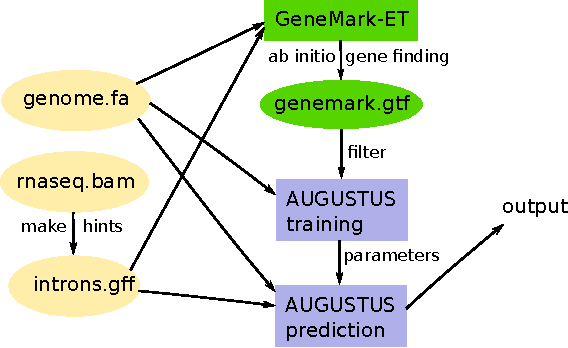
\includegraphics[width=0.7\linewidth]{Figure1.pdf}}
% \caption{Schematic view of the BRAKER1 pipeline.}\label{pipeline}
% \end{figure}
% 
% \begin{table*}[!b]
% \processtable{Accuracy results of BRAKER1 (on softmasked genomes) and MAKER2 (with fully automatic repeat masking, RNA-Seq only source of extrinsic evidence) in genomes of four model organisms. For the fungus \textit{S.~pombe}, we also report accuracy results of CodingQuarry. Accuracy results for BRAKER1 on unmasked genomes can be found in Supplementary Table 2.\label{Tab:01}}
% {\begin{tabular}{lp{.9cm}p{.9cm}p{.9cm}p{.9cm}p{.9cm}p{.9cm}p{.9cm}p{.9cm}p{.9cm}}\toprule
%  & \multicolumn{2}{c}{\textit{Arabidopsis thaliana}} &  \multicolumn{2}{c}{\textit{Caenorhabditis elegans}} &  \multicolumn{2}{c}{\textit{Drosophila melanogaster}} &  \multicolumn{3}{c}{\textit{Schizosaccharomyces pombe}}\\
%  & \tiny{BRAKER1} & \tiny{MAKER2} &  \tiny{BRAKER1} & \tiny{MAKER2}  & \tiny{BRAKER1} & \tiny{MAKER2} &\tiny{BRAKER1} & \tiny{MAKER2} &\tiny{CodingQuarry}\\
%  \midrule
% Gene sensitivity        & \textbf{63.9} & 51.3          & \textbf{55.2} & 41.0 & \textbf{67.0} & 58.0 & 76.7 & 42.8 & \textbf{79.7}\\
% Gene specificity        & 51.9          & \textbf{52.5} & \textbf{55.6} & 30.8 & \textbf{61.0} & 46.9 & \textbf{79.9} & 68.7 & 72.6\\
% Transcript sensitivity  & \textbf{54.6} & 43.5          & \textbf{43.4} & 31.3 & \textbf{49.8} & 42.3 & 76.7 & 42.8 & \textbf{79.7}\\
% Transcript specificity  & 50.7          & \textbf{52.5} & \textbf{53.7} & 30.8 & \textbf{59.8} & 47.9 & \textbf{75.8} & 68.7 & 72.6\\
% Exon sensitivity        & \textbf{82.6} & 76.1          & \textbf{80.2} & 69.4 & \textbf{73.1} & 64.9 & \textbf{82.7} & 50.1 & 79.6\\
% Exon specificity        & \textbf{79.0} & 76.1          & \textbf{85.5} & 62.3 & \textbf{67.0} & 55.0 & \textbf{82.4} & 71.4 & 81.7\\
% \botrule
% 
% \end{tabular}}{}
% \end{table*}

Transcriptome sequencing data, RNA-Seq reads, aligned to a genome sequence have great potential to improve the accuracy of structural genome annotation: spliced alignments may indicate intron positions, and coverage increase and decrease along genomic sequence may indicate locations of exon-noncoding region borders. Nevertheless, RNA-Seq coverage alone is no reliable indicator of protein coding regions \citep{InsectOpinion2015}. 

The prediction of protein coding regions in genomes is often accomplished by tools that use statistical models to discriminate genes from other genomic regions. Some gene prediction tools can additionally use RNA-Seq 
%read alignments
 to improve prediction accuracy.

Statistical models used in gene prediction tools usually require a training  step to identify species specific parameters. For many tools, including AUGUSTUS, the training step has to be performed on a set of example genes generated by a special procedure. In the past, training gene sets have often been produced with help of expressed sequence tags (ESTs) or protein data, and sometimes have been subject to validation by experts. With the rapidly growing number of novel sequenced genomes, this approach becomes infeasible. Fast and fully automated methods for training of gene prediction tools, ideally using the nowadays often available RNA-Seq data, are urgently needed.

In principle, RNA-Seq reads can be assembled into longer contigs, and such contigs can be used similarly to EST data both in training of gene finders and in the prediction step. One of the tools that follow this idea is the MAKER2 pipeline \citep{MAKER2}. However, the RNA-Seq Genome Annotation Assessment Project (RGASP) \citep{RGASP} has shown that transcriptome assembly is prone to errors. To avoid transferring assembly errors into gene prediction, it is advantageous to use the transcript information contained in unassembled mapped reads.

We have developed BRAKER1, a pipeline that combines the advantages of two gene prediction tools: GeneMark-ET \citep{GeneMark-ET} incorporates unassembled RNA-Seq reads into unsupervised training and subsequently generates \textit{ab initio} gene predictions. A subset of genes predicted by GeneMark-ET are used to train AUGUSTUS \citep{AUGUSTUS}. AUGUSTUS lacks an unsupervised training procedure and has an exceptional feature - discriminative training module - that requires a good training set. However, AUGUSTUS incorporates information derived from mapped unassembled RNA-Seq reads into the prediction step; in RGASP, AUGUSTUS was one of the most accurate tools for predicting protein coding genes with RNA-Seq support. We report accuracy results for BRAKER1 on four model organisms and compare to the accuracy of MAKER2. Recently, Testa et al.~published CodingQuarry, a pipeline for RNA-Seq assembly supported training and gene prediction, but recommend its application only to fungi \citep{CodingQuarry}. Therefore, we 
include CodingQuarry into the comparison on \textit{Schizosaccharomyces pombe}.


\begin{methods}
\section{Methods}

BRAKER1 is implemented in Perl and requires two input files: an RNA-Seq alignment file in \texttt{bam}-format, and a corresponding genome file in \texttt{fasta}-format. Spliced alignment information is extracted from the RNA-Seq file and stored in \texttt{GFF}-format. GeneMark-ET uses the genome file and  the spliced alignment \texttt{GFF}-file for RNA-Seq supported unsupervised training. After training, GeneMark-ET creates an \textit{ab initio} gene set. Those gene structures that have support by RNA-Seq alignments in all introns are selected for automated training of AUGUSTUS. After training, AUGUSTUS predicts genes in the input genome file using spliced alignment information from RNA-Seq as extrinsic evidence. The pipeline is illustrated in Supplementary Figure 2.1.



%\section{Test Data}

In order to demonstrate prediction accuracy, nuclear genomes, reference annotations and RNA-Seq libraries were retrieved for four model organisms \textit{Arabidopsis thaliana}, \textit{Caenorhabditis elegans}, \textit{Drosophila melanogaster}, and \textit{Schizosaccharomyces pombe} were retrieved from databases specified in Supplementary.

Presence of repetitive sequences and mobile elements (transposable elements, TEs) is a characteristic feature of eukaryotic genomes. Repetitive sequences create challenges for automatic gene finders both at parameter estimation step and gene prediction step. The size and quality of the training set generated by GeneMark-ET for AUGUSTUS (multi-exons genes with so called anchored introns, the introns predicted ab initio and also supported by RNA-Seq mapping) is not significantly affected by TEs masking since TEs have no anchored introns. However, at the prediction step TEs can corrupt gene prediction. For this reason, soft masking of genomic sequence is recommended before execution of BRAKER1. In this publication we used RepeatModeler to generate repeat library and RepeatMasker to mask sequence [Smit, A.F.A. and Hubley, R. (2008-2015) RepeatModeler Open-1.0, \url{http://www.repeatmasker.org/}].

\end{methods}


\section{Results and Discussion}

\begin{table*}[!t]
\processtable{\textcolor{red}{Accuracy results of the final gene prediction step of BRAKER1 with AUGUSTUS (on softmasked genomes) and MAKER2 (with fully automatic repeat masking, RNA-Seq only source of extrinsic evidence) in genomes of four model organisms. For the fungus \textit{S.~pombe}, we also report accuracy results of CodingQuarry. Accuracy results for BRAKER1 on unmasked genomes can be found in Supplementary Table 1.2.}\label{Tab:01}}
{\begin{tabular}{lp{.9cm}p{.9cm}p{.9cm}p{.9cm}p{.9cm}p{.9cm}p{.9cm}p{.9cm}p{.9cm}}\hline
 & \multicolumn{2}{c}{\textit{Arabidopsis thaliana}} &  \multicolumn{2}{c}{\textit{Caenorhabditis elegans}} &  \multicolumn{2}{c}{\textit{Drosophila melanogaster}} &  \multicolumn{3}{c}{\textit{Schizosaccharomyces pombe}}\\
 & \tiny{BRAKER1} & \tiny{MAKER2} &  \tiny{BRAKER1} & \tiny{MAKER2}  & \tiny{BRAKER1} & \tiny{MAKER2} &\tiny{BRAKER1} & \tiny{MAKER2} &\tiny{CodingQuarry}\\
 \hline
Gene sensitivity        & \textbf{64.4} & 51.3          & \textbf{55.0} & 41.0 & \textbf{67.6} & 58.0 & 77.2 & 42.8 & \textbf{79.7}\\
Gene specificity        & 52.0          & \textbf{52.5} & \textbf{55.2} & 30.8 & \textbf{61.1} & 47.9 & \textbf{80.7} & 68.7 & 72.6\\
Transcript sensitivity  & \textbf{55.0} & 43.5          & \textbf{43.0} & 31.3 & \textbf{50.2} & 42.3 & 77.2 & 42.8 & \textbf{79.7}\\
Transcript specificity  & 50.9          & \textbf{52.5} & \textbf{53.2} & 30.8 & \textbf{59.9} & 47.9 & \textbf{76.6} & 68.7 & 72.6\\
Exon sensitivity        & \textbf{82.9} & 76.1          & \textbf{80.2} & 69.4 & \textbf{73.3} & 64.9 & \textbf{82.7} & 50.1 & 79.6\\
Exon specificity        & \textbf{79.0} & 76.1          & \textbf{85.3} & 62.3 & \textbf{67.3} & 55.0 & \textbf{83.3} & 71.4 & 81.7\\
\hline
\end{tabular}}{}
\end{table*}

When comparing BRAKER1 to MAKER2 (details on the MAKER2 run are described in Supplementary), BRAKER1 gains on average $~$15 percent points in accuracy on gene level\footnote{A \textit{gene} may have several \textit{transcripts} in the reference and in a predicted gene set. When computing \textit{transcript} level accuracy, each transcript variant is counted as a TP/FP/FN on its own. When computing \textit{gene} level accuracy, a predicted gene is counted as TP if at least one of its transcripts matches correctly a reference transcript. For details, see documentation of the EVAL package \citep{Eval}} when compared to MAKER2 (see \textcolor{red}{table \ref{Tab:01}}).
%One could ask - which factors are behind better performance of BRAKER1 in comparison with MAKER2. BRAKER1 is using RNA-Seq assisted GeneMark-ET \citep{GeneMark-ET}  instead of purely ab initio self-training GeneMark-ES \citep{GeneMark-ES}. GeneMark-ET performance improves with respect to GeneMark-ES on larger genomes having longer introns and intergenic regions. On shorter genomes, such as fungal ones, the difference is marginal. 
We should remind that the comparison of accuracy does not consider the capability of MAKER2 to use a protein database. BRAKER1 currently does not use a protein database. 
%In addition, benchmarking a homology based annotation method for a realistic annotation project is difficult because the information gain from using a protein database strongly depends on the phylogenetic distance of the target species to species in the database and their annotation quality. 
The RNA-Seq approach used here is independent of a database.

Notably, \citet{SnowyOwl} developed a pipeline, SnowyOwl, with GeneMark-ES \cite{GeneMark-ES} and AUGUSTUS to predict genes in fungal genomes. SnowyOwl attempts to improve prediction accuracy by selecting a gene variant with the highest homology score from a set of predicted gene variants in the same locus. This pipeline requires protein database information as additional external resource.  We did not include SnowyOwl into comparisons since it cannot work without protein information.% which we do not admit for usage in this study. 

Since BRAKER1 uses AUGUSTUS being trained on GeneMark-ET, and since AUGUSTUS incorporates RNA-Seq into the prediction step, we expect to see an increase in accuracy when comparing AUGUSTUS to GeneMark-ET. This is the case for \textit{A.~thaliana}, \textit{C.~elegans} and \textit{D.~melanogaster}; on the fungus \textit{S.~pombe}, GeneMark-ET is superior to AUGUSTUS in the current version of BRAKER1 (see Supplementary Table \textcolor{red}{1.1}). 
%AUGUSTUS parameters can be adapted to improve prediction accuracy in such species, but we here report results with the BRAKER1 default settings. 

Supplementary Table 1.2 shows that genome repeat masking is an optional pre-processing step for running BRAKER1 that does not affect prediction accuracy much. We observed that on \textit{S.~pombe}, BRAKER1 is on average $\sim$4\% more accurate on gene level than CodingQuarry. %Notably, GeneMark-ET alone is even more accurate on this species. 
BRAKER1 required $\sim$17.5 hours on a single CPU for training and prediction on \textit{D.~melanogaster} but can be run in parallel.

In conclusion, BRAKER1 is a fully automatic eukaryotic gene prediction pipeline with GeneMark-ET and AUGUSTUS working with genomic and RNA-Seq read information. In contrast to MAKER2, BRAKER1 is a ``one step process'', meaning that after starting it once, it will execute training and prediction without the need for manual command execution. BRAKER1 predicts genes more accurately than MAKER2 and CodingQuarry.



\section*{Acknowledgement}

We would like to thank Mark Yandell and Carson Holt for valuable advice on running MAKER2.

\paragraph{Funding\textcolon} This work is supported by the US National Institutes of Health grant HG000783.

%\bibliographystyle{natbib}
%\bibliographystyle{achemnat}
%\bibliographystyle{plainnat}
%\bibliographystyle{abbrv}
%\bibliographystyle{bioinformatics}
%
%\bibliographystyle{plain}
%
%\bibliography{Document}


\begin{thebibliography}{}
\bibitem[Hoff and Stanke, 2015]{InsectOpinion2015}Hoff, K.J. and Stanke, M. (2015) Current Methods for Automated Annotation of Protein-Coding Genes, {\it Current Opinion in Insect Science}, doi:10.1016/j.cois.2015.02.008.

\bibitem[Steijger {\it et~al}., 2013]{RGASP} Steijger,T. and Abril,J.F. and Engstr\"{o}m,P.G. and Kokocinski,F. and The RGASP Consortium, Hubard,T.J. and Guigo,R. and Harrow, J. and Bertone, P. (2013) Assessment of transcript reconstruction methods for
 RNA-seq, {\it Nature Methods}, doi:10.1038/nmeth.271.

\bibitem[Lomsadze {\it et~al}., 2014]{GeneMark-ET} Lomsadze, A. and Burns, P.D. and Borodovsky, M. (2014) Integration of mapped RNA-Seq reads into automatic training of eukaryotic gene finding algorithm, {\it Nucleic Acids Research}, doi:10.1093/nar/gku557.

\bibitem[Ter-Hovhannisyan {\it et~al}., 2008]{GeneMark-ES} Ter-Hovhannisyan, V. and Lomsadze, A. and Chernoff, Y. and Borodovsky, M. (2008) Gene prediction in novel fungal genomes using an ab initio algorithm with unsupervised training, \textit{Genome Research}, \textbf{18}(12):1979-90.

\bibitem[Stanke \textit{et~al}., 2008]{AUGUSTUS}
Stanke, M. and Diekhans, M. and Baertsch, R. and Haussler, D. (2008) Using native and syntenically mapped cDNA alignments to improve de novo gene finding, \textit{Bioinformatics}, \textbf{24}(5), 637.

\bibitem[Holt and Yandell, 2011]{MAKER2} Holt, C. and Yandell, M. (2011) MAKER2: an annotation pipeline and genome-database management tool for second-generation genome projects, \textit{BMC Bioinformatics}, \textbf{12}:491.

\bibitem[Testa \textit{et~al}., 2015]{CodingQuarry} Testa, A.C. and Hane, J.K. and Ellwood, S.R. and Oliver R.P. (2015) CodingQuarry: highly accurate hidden Markov model gene prediction in fungal genomes using RNA-seq transcripts, \textit{BMC Genomics} \textbf{16}:170.

%\bibitem[Smit and Hubley, 2015]{RepeatModeler} Smit, A.F.A. and Hubley, R. (2008-2015) RepeatModeler Open-1.0 \textit{\url{http://www.repeatmasker.org}}.

\bibitem[Keibler and Brent, (2003)]{Eval} Keibler, E. and Brent, M.R. (2003) Eval: a software package for analysis of genome annotations, \textit{BMC Bioinformatics} \textbf{4}:50.

\bibitem[Reid \textit{et~al}., 2014]{SnowyOwl}Reid, I. and O'Toole, N. and Zabaney, O. and Nourzadesh, R. and Dahdouli, M. and Abdellateef, M. and Gordon, P.M.K. and Soh, J. and Butler, G. and Sensen, C. W. and Tsang, A. (2014) SnowyOwl: accurate prediction of fungal genes by using RNA-Seq and homology information to select among ab initio models, \textit{BMC Bioinformatics} \textbf{15}:229.

%\bibitem[Haas \textit{et~al}., 2008] Haas, B. and Salzberg, S. and Zhu, W. and Pertea, M. and Allen, J. and Orvis, J. and White, O. and Buell, C.R. and Wortman, J. (2008) Automated eukaryotic gene structure annotation using EvidenceModeler and the program to assemble spliced reads, {\it Genome Biology}, \textbf{9}(1):R7.

%\bibitem[Keller \textit{et~al}., 2008] Keller, O. and Odronitz, F. and Stanke, M. and Kollmar, M. and Waack, S. (2008) Scipio: Using protein sequences to determine the precise exon/intron structures of genes and their orthologs in closely related species, {\it BMC Bioinformatics}, \textbf{9}(1):278.

\end{thebibliography}
\end{document}
